\section{Introduction}
\label{sec:introduction}

% state the learning objective
\par The objective of this laboratory assignment is to study a circuit containing an
AC voltage source $V_S$ and a capacitor connected to seven resistors $R_{1-7}$, a linear voltage-controlled current source and a  linear current-controlled voltage source. The circuit can be seen in Figure~\ref{fig:rc}.\\



In Section~\ref{sec:analysis}, it was used the node analysis methods to solve the circuit for $t<0$. It was also determined the equivalent resistance Req as seen from the capacitor terminals. After that it was calculated the natural and forced solutions for the voltage in node 6. Finally, it was analysed the response to frequency variation.
In Section~\ref{sec:simulation}, the circuit is analysed by
simulation, and the results are compared to the theoretical results obtained in
Section~\ref{sec:analysis}. The conclusions of this study are outlined in
Section~\ref{sec:conclusion}.

\begin{figure}[h] \centering
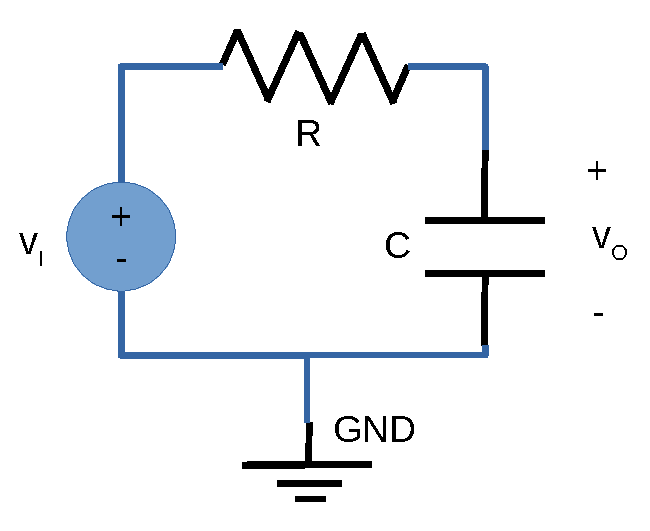
\includegraphics[width=0.6\linewidth]{rc.pdf}
\caption{RC Circuit}
\label{fig:rc}
\end{figure}
